\documentclass[a4paper,11pt]{article}
\usepackage{amssymb}
\usepackage{geometry}
\usepackage{amsmath}
\usepackage{graphicx}
\usepackage{hyperref}
\usepackage{subcaption}
\hypersetup{colorlinks = true}
\geometry{left=25mm,right=25mm,%
bindingoffset=0mm, top=20mm,bottom=20mm}
\renewcommand{\baselinestretch}{1}
\usepackage{multicol}
\usepackage{indentfirst}
\usepackage{dirtytalk}

\title{Energy labeled houses VS Energy consumption}
\author{}
\date{09 January 2021}

\begin{document}

\maketitle

\section{Introduction}

What is an energy labeled house? Energy labeled houses are the houses that are a label with a letter grade on how efficient the energy is being used in that particular house. For example, a house with an A++ grade would have the least amount of energy lost when using electricity, heaters, gas, and so on. The house with a G grade will have the most amount of energy lost and for sustainability reasons, it would be better to have a house with an A++ grade rather than G grade. If more houses are graded with higher labels, will there be a reduction in energy consumption? Even if less energy is lost, it does not necessarily mean that less energy is consumed. If the number of people living in a house is more than 30, then the average energy consumption for that household would still be higher than a house with 10 people, whether they lived in an A++ grade house or not. However, one can also assume that as less energy is lost, the energy is consumed efficiently. Then, less energy is needed for functioning the houses, which will in return reduce the energy consumption. Assuming that they use the same energy unit to function the house, it can be said that an A++ house with 20 people living in it will consume less energy than a G house with 20 people living in it. Although there is a correlation, the question remained: would the energy consumption varied as the number of labeled houses increase? 

\section{Methods}
The data used in this analysis is obtained from Rijkswaterstaat \cite{Rijkswaterstaat} and it only consists of cities in the Netherlands. The data are collected for monitoring the climate in the country. A few variables from that dataset are selected to answer the aforementioned question. Firstly, the total number of labeled houses are plotted against year to see if there is any change in the number of houses being labeled, as seen in \autoref{fig:my_label1}. Secondly, a graph with the number of houses for each label is plotted to observe the trends lest some changes in one label might affect the amount of energy consumed. (as shown in \autoref{fig:image2}).  Lastly, the average energy consumption per house was taken and plotted against year to see how the energy consumption has varied across the year, regardless of whether they are A++ graded or G graded or unlabelled (\autoref{fig:my_label2}). Note that the unit of the natural gas is converted into \emph{kWh} for better comparison with electricity. The number of people in a house is ignored in the analysis and is assumed to be constant for every house.  

\section{Results}
As seen in \autoref{fig:my_label1}, the total number of labeled houses has only been increasing from 2008 to 2019. There has been no drop in between the year. However, when looked closely at \autoref{fig:image2}, there is a drop in the number of houses for several labels, such as D and E, after 2017. Although the number of houses labeled with C's is higher than others, it is also decreasing gradually after 2017.  The number of houses labeled with A++ and A+ grade is very little; moreover so after 2017 (\autoref{fig:subim2}). The number of houses labeled with A's and B's increase across the year. 

On the other hand, when looking at \autoref{fig:my_label2}, the average energy used per house decreased in the period 2008-2019. Although there was an increase in usage of electricity between the year 2008-2010, the general trend was seen on the graph is downward. 


\section{Discussion}

When only comparing \autoref{fig:my_label1} and \autoref{fig:my_label2}, a relation between the increase in labeled houses and the decrease in energy consumption can be formed. As the number of labeled houses increases, there are more known houses using energy efficiently. At the same time, the average energy consumption per house is decreasing as well. By just looking at the two graphs, one can mistakenly think that the two are related to each other: the energy consumption will decrease when the number of energy labeled houses increase. However, it is important to know that the energy labeled houses are only the house with a label; an unlabeled house will not mean that it is not using the energy efficiently. Although there is a correlation between the two (as given with examples in the introduction section), the energy consumption does not vary with the increase in the number of label houses. They could also be seen on graphs when comparing \autoref{fig:image2} and \autoref{fig:my_label2}. During the period where there are drops for several labels after 2017, there are no changes in energy consumption after 2017. There has only been a constant decrease in energy consumption regardless of the ups and downs. Thereafter, it can be concluded that energy consumption does not change with the change in the number of labeled houses. 

\section{Conclusion}
At a glance, it can be observed that the energy consumption might be varying with how the number of labeled houses changes. However, after looking at a graph for each label and remembering the definition of the energy-labeled houses, it is found that they are not related at all and the energy consumption might be varying due to other factors such as the number of people in the house. 

\begin{figure}
    \centering
    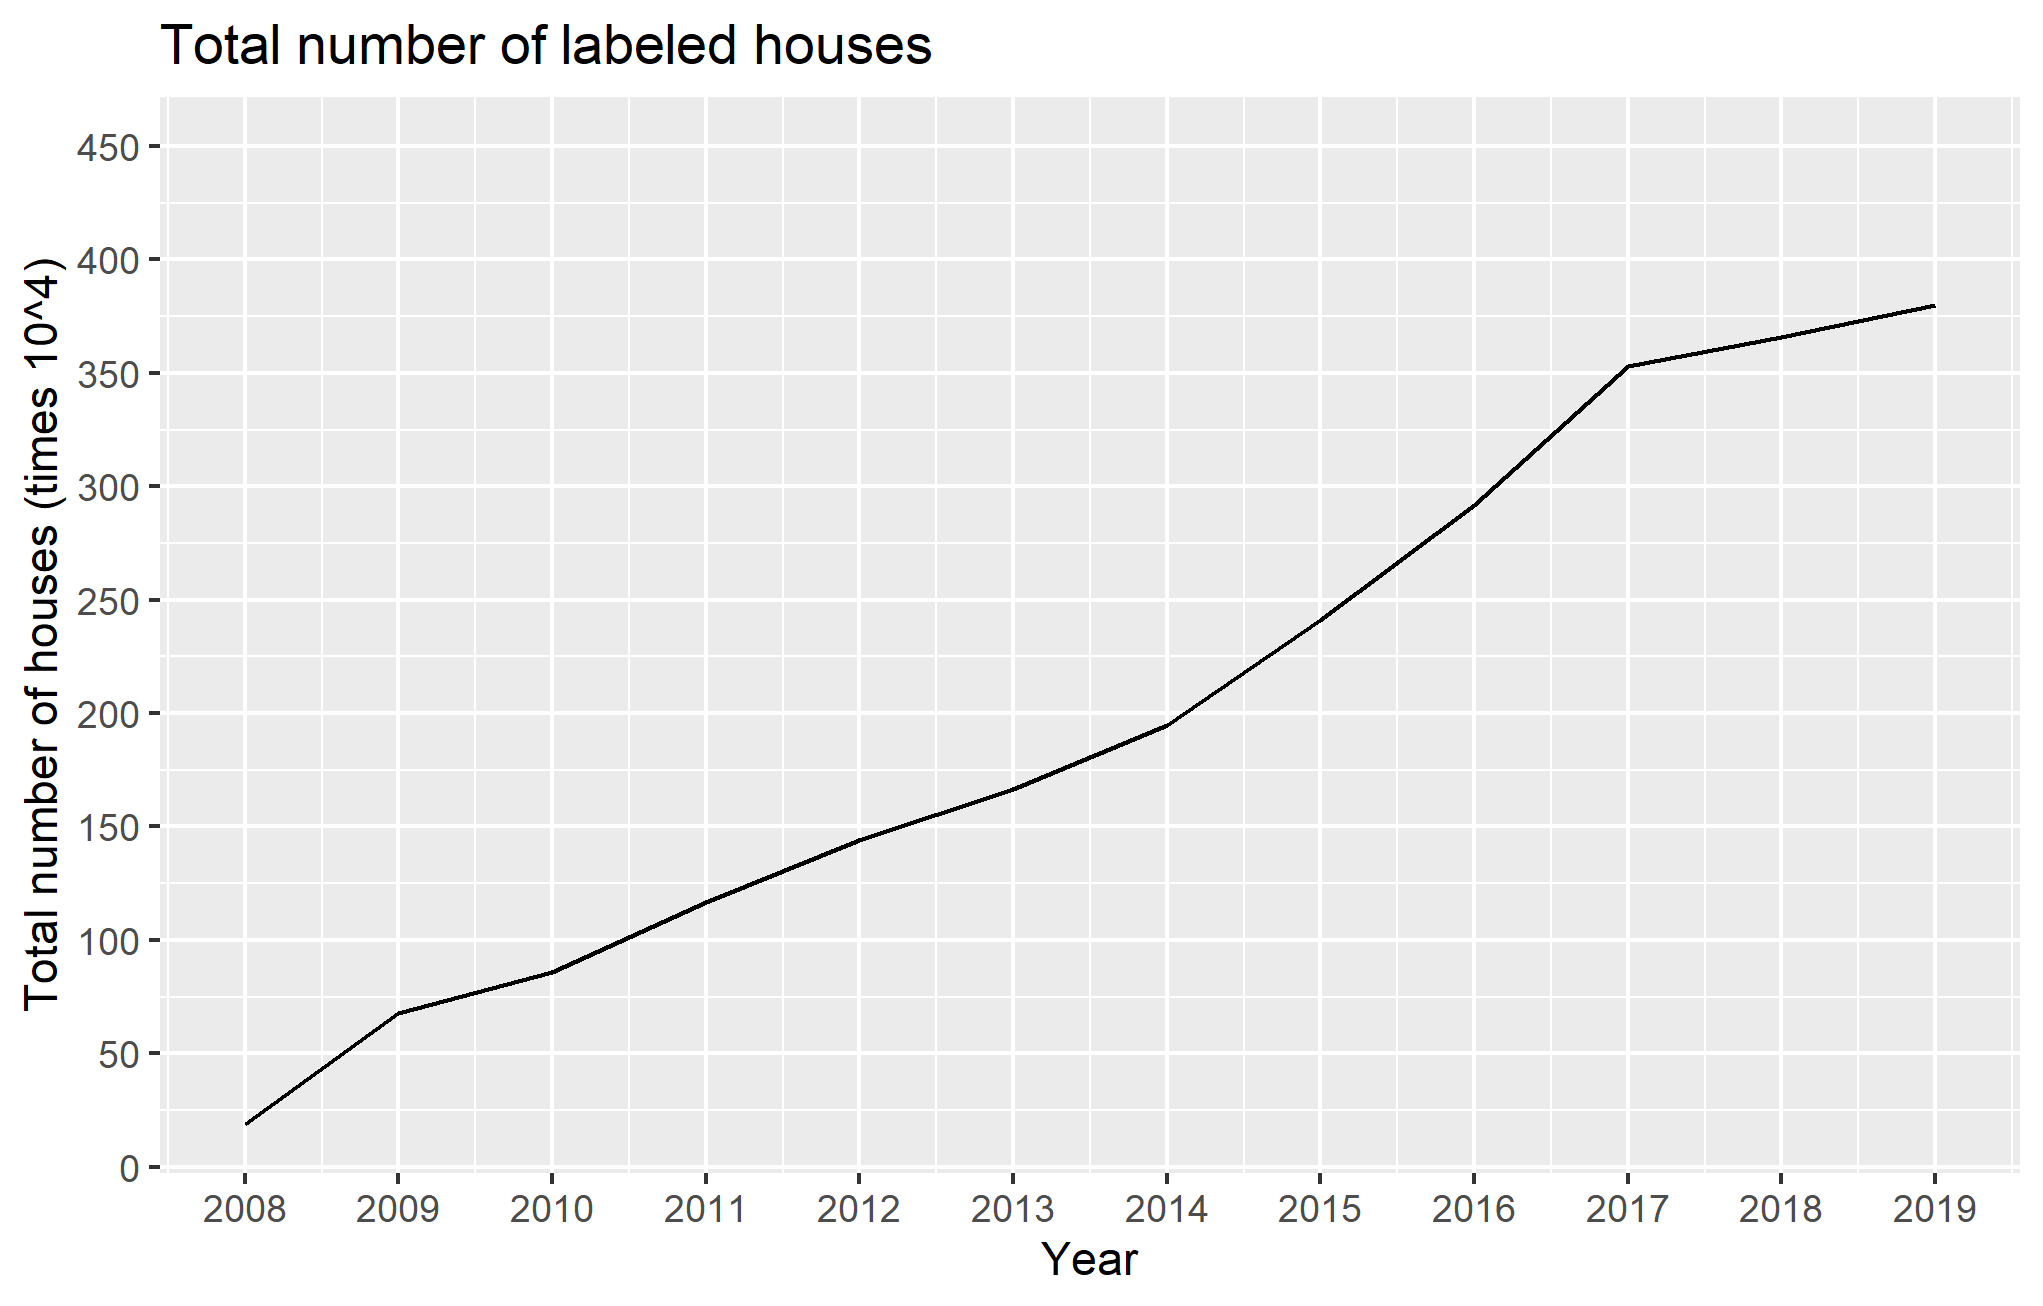
\includegraphics[width=\textwidth]{Tot number of labeled houses.png}
    \caption{Total number of labelled houses from 2008 to 2019}
    \label{fig:my_label1}
\end{figure}    
\begin{figure}
\begin{subfigure}{0.5\textwidth}
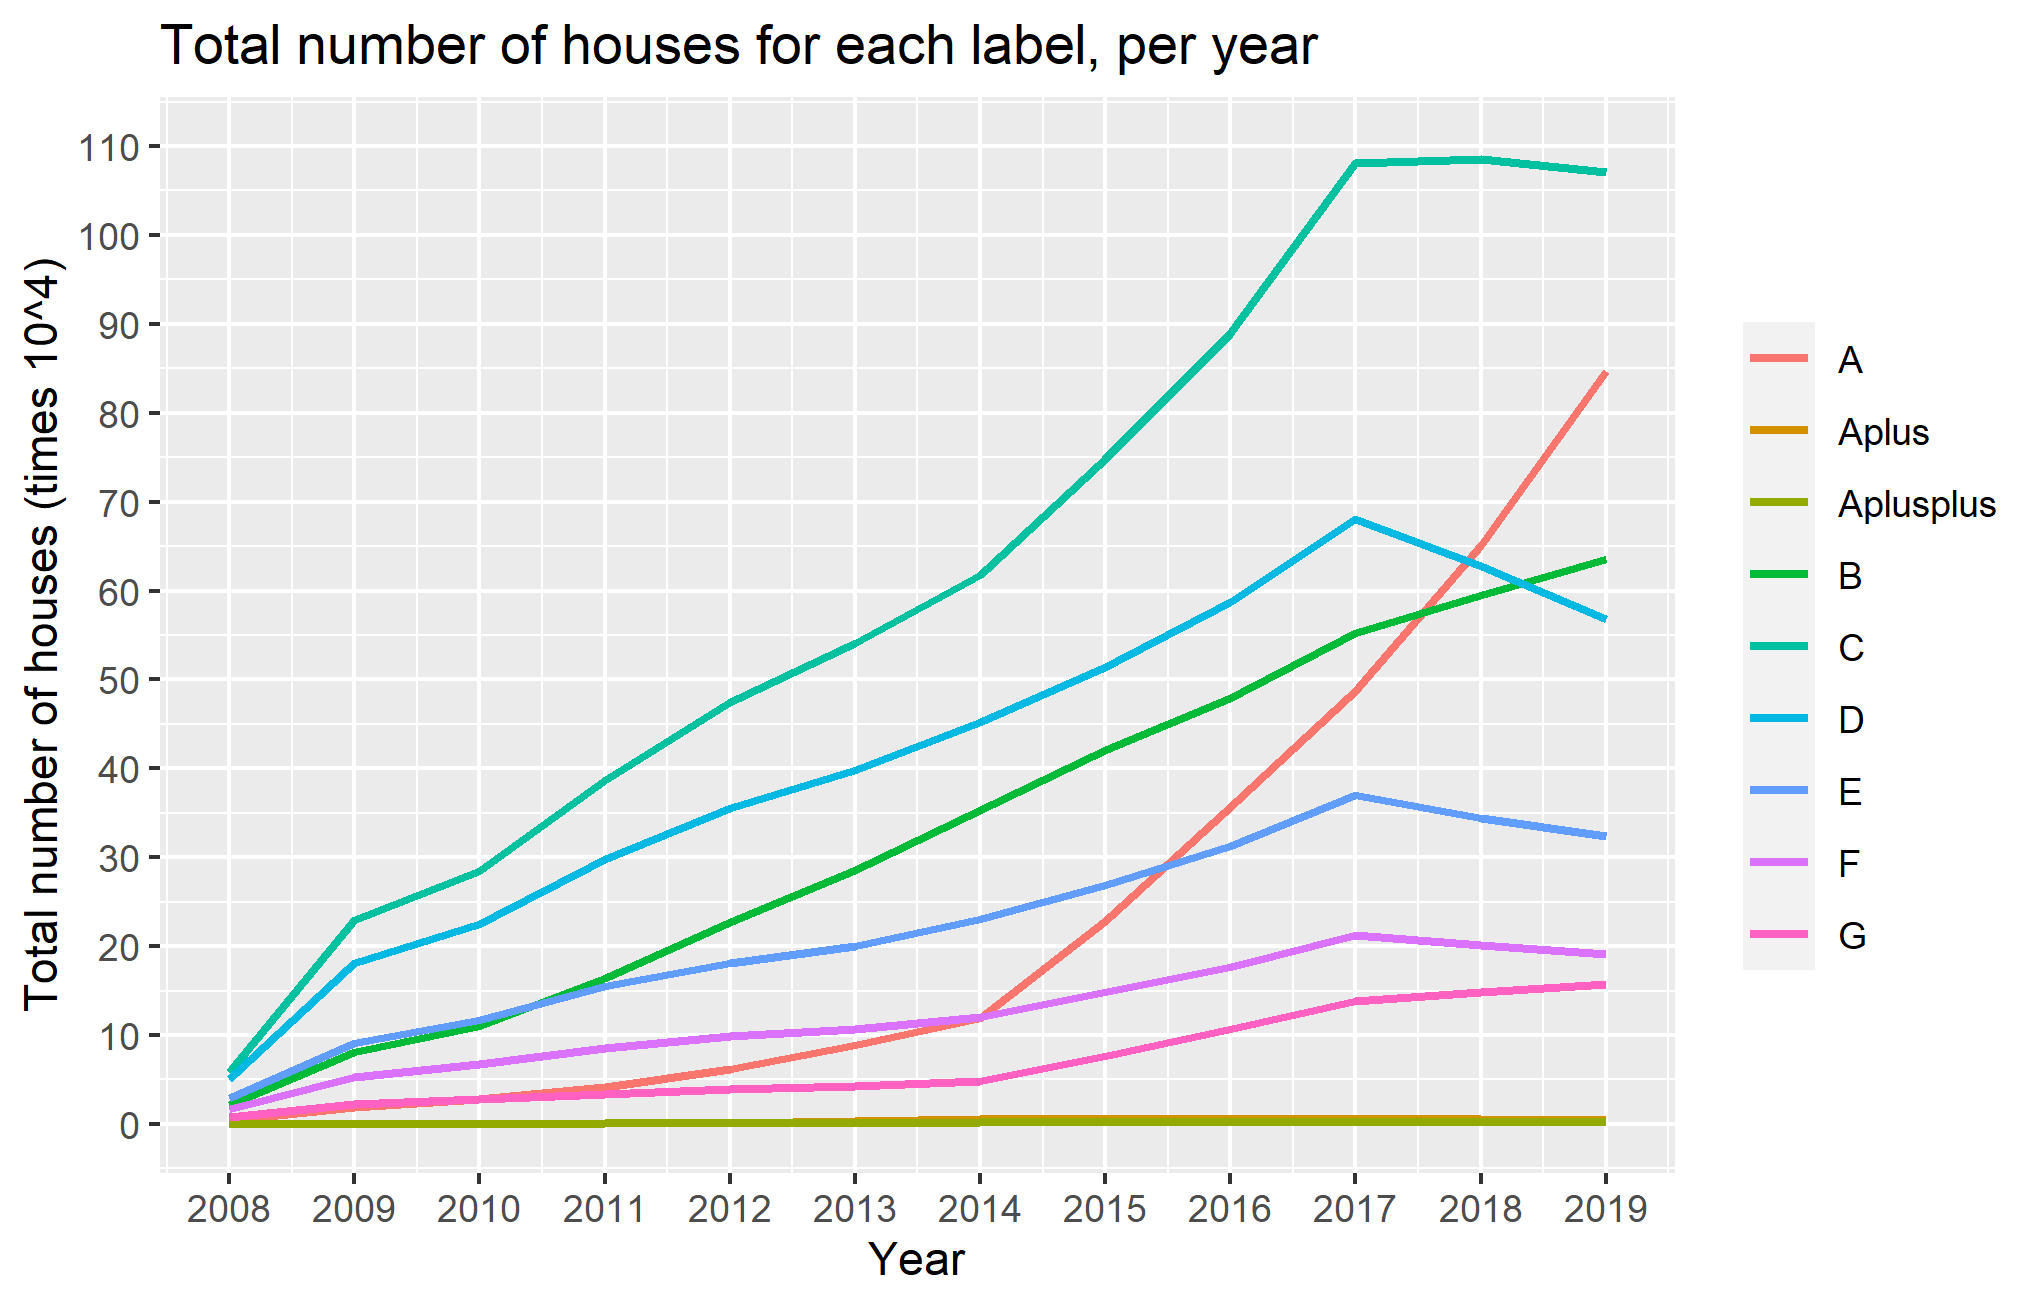
\includegraphics[width=\linewidth]{Tot no. of houses for each label, per year.png} 
\caption{Total number of houses for each label}
\label{fig:subim1}
\end{subfigure}
\begin{subfigure}{0.5\textwidth}
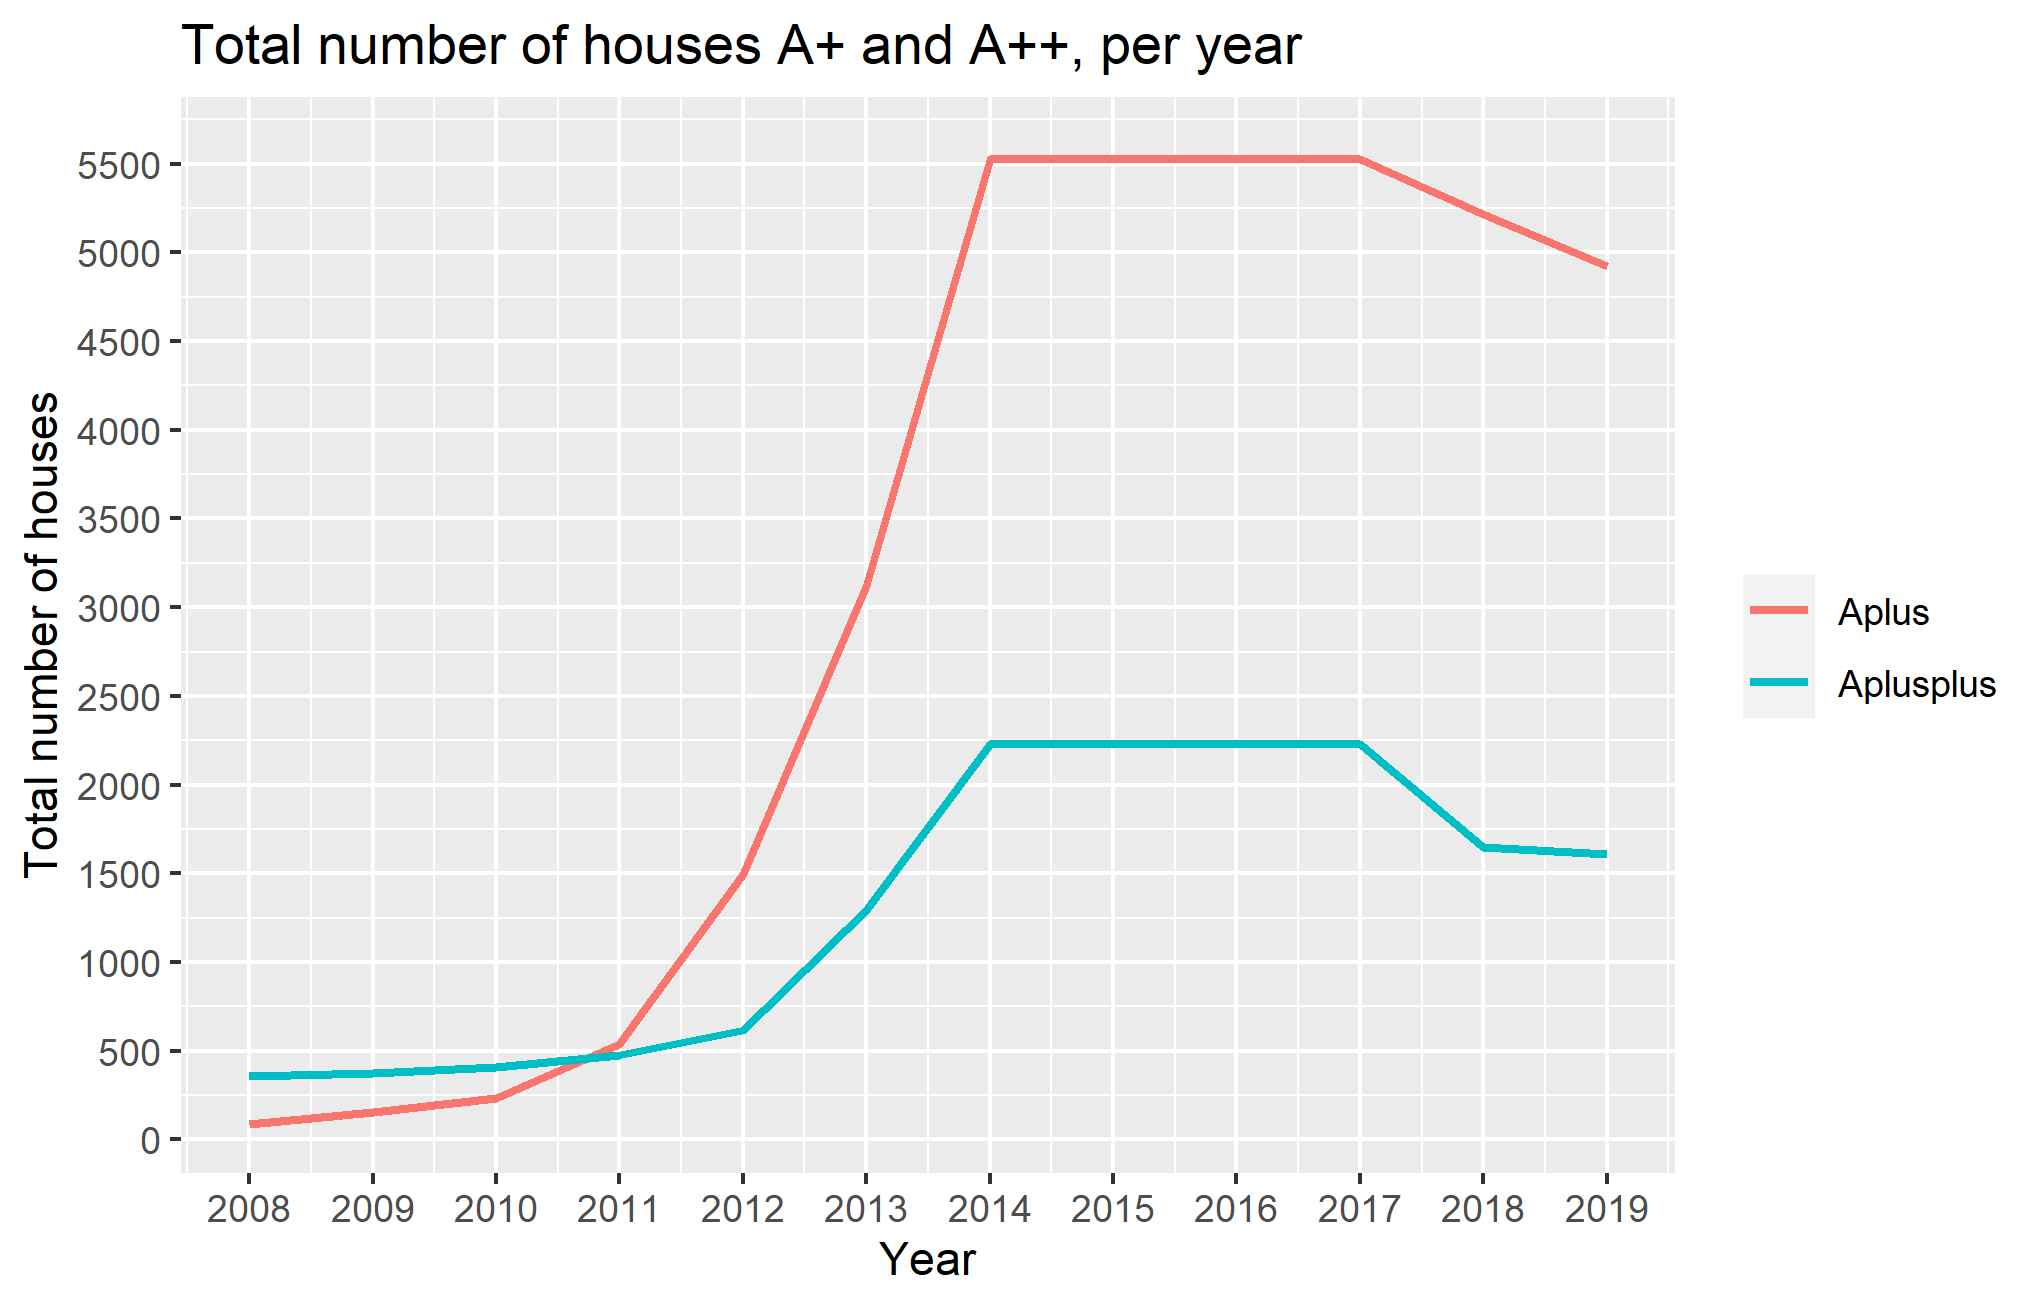
\includegraphics[width = \linewidth]{A closeup view for A+ and A++.png}
\caption{A close-up inspection for A+ and A++ labels}
\label{fig:subim2}
\end{subfigure}

\caption{Total number of houses for every label from 2008 to 2019}
\label{fig:image2}
\end{figure}
\begin{figure}
    \centering
    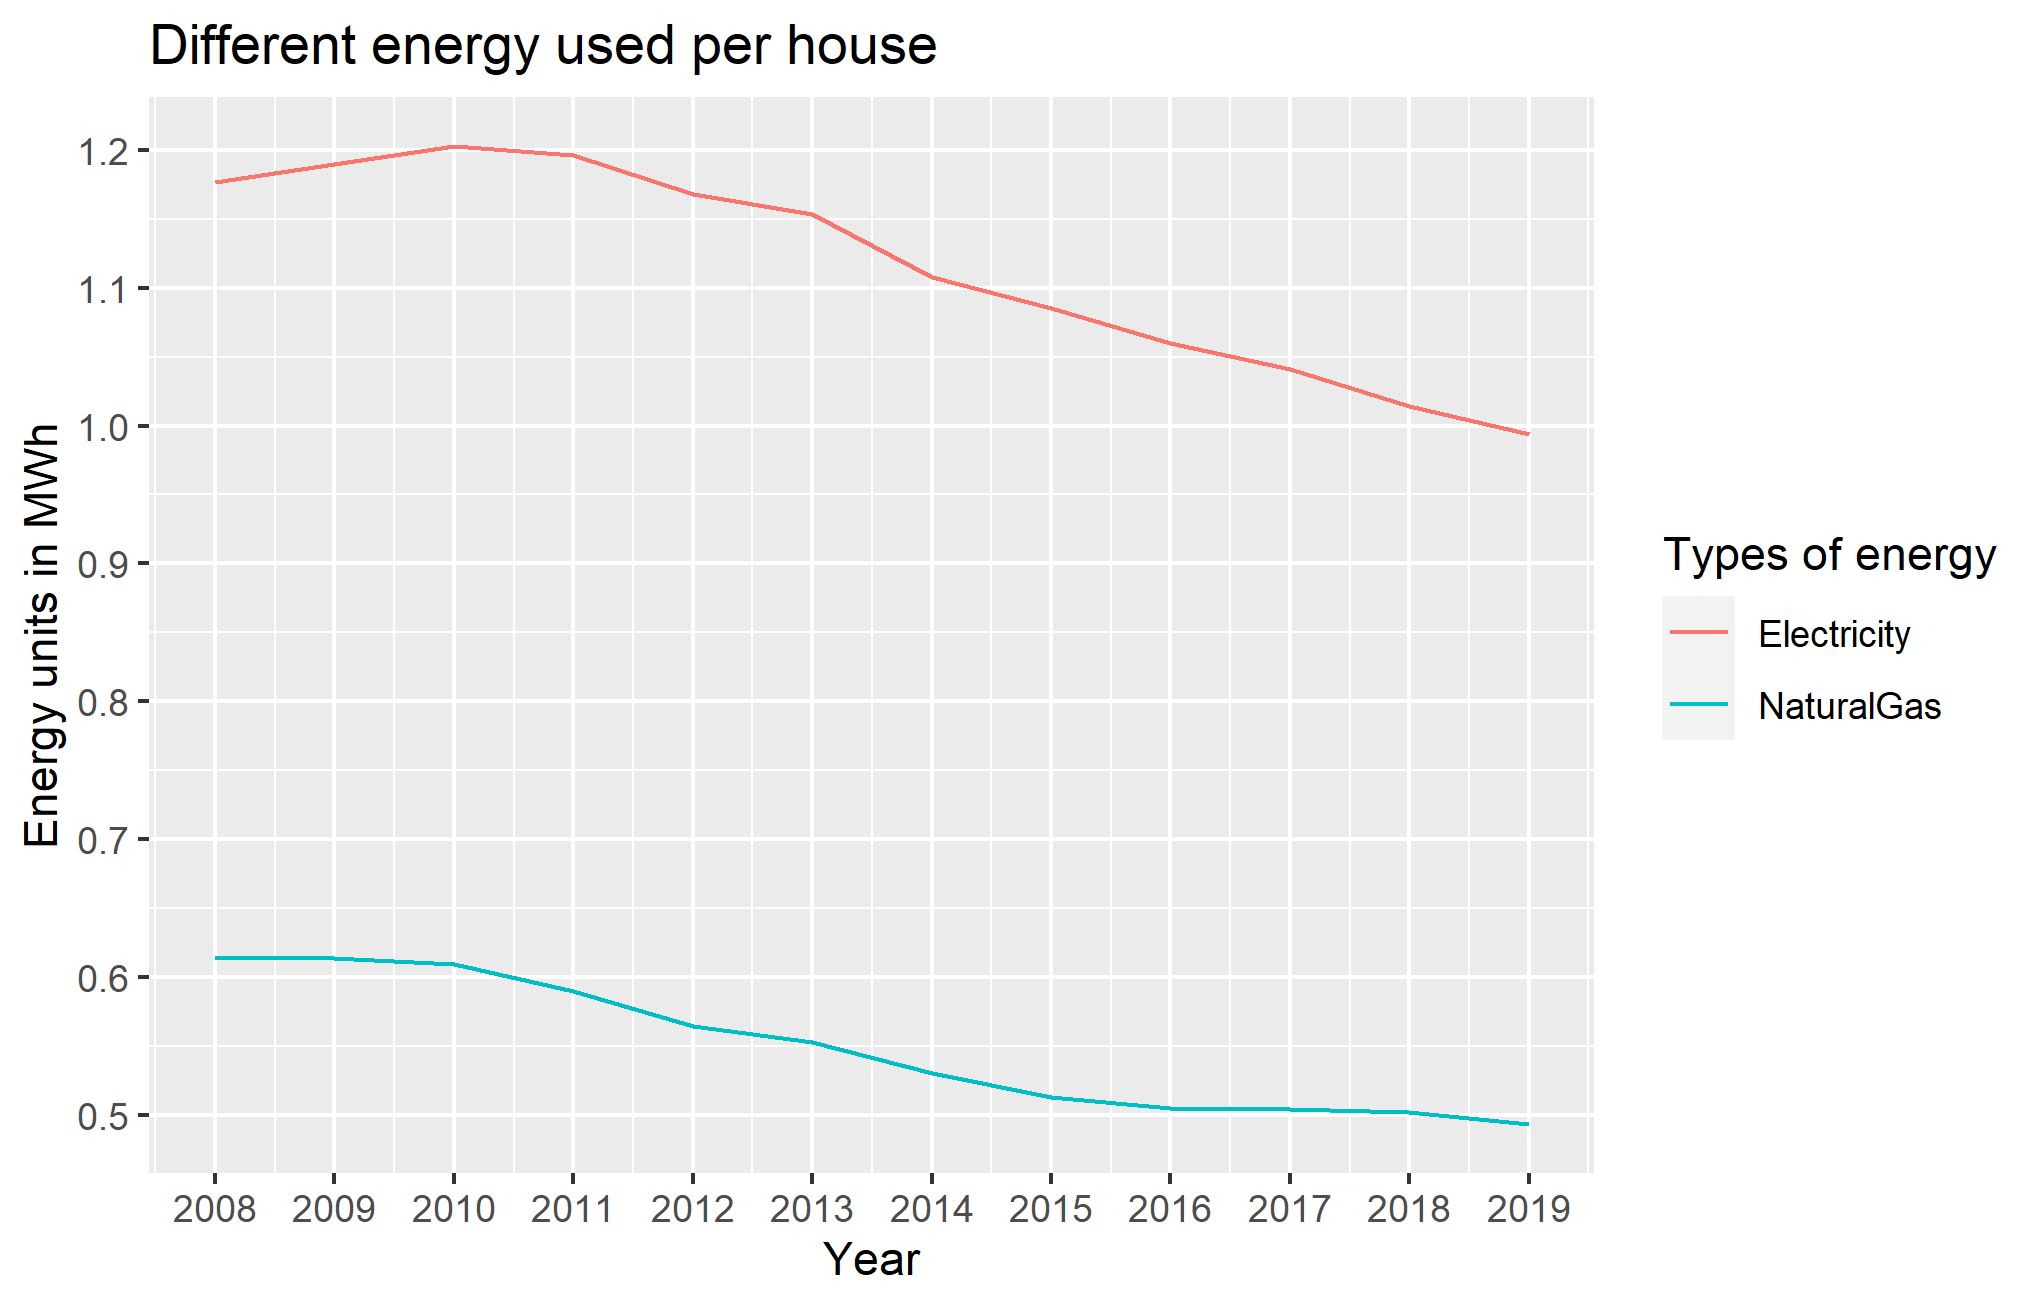
\includegraphics[width= \textwidth]{Different energy used per house.png}
    \caption{Average energy used per house}
    \label{fig:my_label2}
\end{figure}


\begin{thebibliography}{}
\bibitem{Rijkswaterstaat}
Rijkswaterstaat (Ministerie van Infrastructuur en Waterstaat) (2020). \textit{Climate monitor}
\url{https://klimaatmonitor.databank.nl/dashboard}

\end{thebibliography}

\end{document}
